\section{Introdução ao estudo das funções}

\subsection{Sistemas de coordenadas}

\subsubsection{Sistema cartesiano ortogonal de coordenadas}

O Sistema de coordenadas, mais conhecido como Plano Cartesiano, foi criado por 
René Descartes com o objetivo de localizar pontos. Ele é formado por dois eixos 
perpendiculares: um horizontal e outro vertical que se cruzam na origem das coordenadas. 
O eixo horizonal($0x$) é chamado de \textit{abscissa} e o vertical($0y$) chamado de ordenada. Os eixos 
são enumerados compreendendo o conjunto dos números reais. Observe a seguir a representação do 
Plano Cartesiano:

\begin{center}
  \begin{tikzpicture}
    \tkzInit[xmin=-5, xmax=5, xstep=1, ymin=-5, ymax=5, ystep=1]
    \tkzLabelX[orig=false]
    \tkzLabelY[orig=false]
    \tkzDrawXY
  \end{tikzpicture}
\end{center}

Para determinar as coordenadas do ponto \textit{P} da figura a seguir, traçamos por \textit{P} as 
perpendiculares ao eixo \textit{x} e ao eixo \textit{y}, obtendo, nesses eixos, dois números chamados 
de \textbf{abscissa} e \textbf{ordenada} do ponto \textit{P}, respectivamente.

\begin{center}
  \begin{tikzpicture}[scale=.7]
    \tkzInit[xmin=-5, xmax=5, xstep=1, ymin=-5, ymax=5, ystep=1]
    \tkzLabelX[orig=false]
    \tkzLabelY[orig=false]
    \tkzDrawXY
    \tkzDefPoint(5,4){P}
    \tkzDrawPoints(P)
    \tkzLabelPoint[right](P){$P$}
    \tkzPointShowCoord(P)
  \end{tikzpicture}
\end{center}

No exemplo, as \textbf{coordenadas} do ponto \textit{P} são 5 e 4. A \textbf{abscissa} é 5, e a \textbf{ordenada} é 4. 
Indicamos esse fato por $P(5,4)$.

A representação $(5,4)$ é chamada de ``\textbf{par ordenado} de abscissa 5 e ordenada 4''.

\begin{proposition}{Generalidades}{generalities}
  \begin{enumerate}
    \item Dois pares ordenados de números reais são iguais se, e somente se, suas abscissas são iguais e 
      suas ordenadas são iguais, isto é:

      \vspace{.2cm}
      $(a, b) = (c, d) \iff  a = c \text{ e } b = d$

      \vspace{.2cm}
      Por exemplo:

      \vspace{.2cm}
      $(a, 8) = (7, y) \iff a = 7 \text{ e } y = 8$

    \vspace{.2cm}
    \item Os eixos $0x$ e $0y$, chamados de \textbf{eixos coordenados}, separam o plano cartesiano em quatro 
      regiões denominadas \textbf{quadrantes}, que devem ser enumerados conforme a figura:

    \vspace{.2cm}
    \begin{center}
      
\begin{tikzpicture}[scale=.7]
        \tkzInit[xmin=-10, xmax=10, xstep=1, ymin=-5, ymax=5, ystep=1]
        \tkzDrawXY[noticks]
        \tkzDefPoint(5,3){A}
        \tkzDefPoint(-5,3){B}
        \tkzDefPoint(-5,-3){C}
        \tkzDefPoint(5,-3){D}
        \tkzText[color = black](A){Primeiro Quadrante ($Q_1$)}
        \tkzText[color = black](B){Primeiro Quadrante ($Q_2$)}
        \tkzText[color = black](C){Primeiro Quadrante ($Q_3$)}
        \tkzText[color = black](D){Primeiro Quadrante ($Q_4$)}
      \end{tikzpicture}
    \end{center}

    \vspace{.2cm}
    \begin{tasks}(2)
      \task[] $P(a,b) \in Q_1 \iff a > 0 \text{ e } b > 0$
      \task[] $P(a,b) \in Q_2 \iff a < 0 \text{ e } b > 0$
      \task[] $P(a,b) \in Q_3 \iff a < 0 \text{ e } b < 0$
      \task[] $P(a,b) \in Q_4 \iff a > 0 \text{ e } b < 0$
    \end{tasks}

    \vspace{.2cm}
    Por exemplo:

    \vspace{.2cm}
    \begin{tasks}(2)
      \task[\#] $(4,2) \in Q_1$
      \task[\#] $(-\frac{1}{2},9) \in Q_2$ 
      \task[\#] $(-3,-5) \in Q_3$
      \task[\#] $(\frac{3}{2},-1) \in Q_4$
    \end{tasks}

    Os pontos dos eixos coordenados não pertencem a nenhum quadrante.

    \item Todo ponto de abscissa nula (igual a zero) pertence ao eixo $Oy$, e todo ponto de ordenada nula 
      (igual a zero) pertence ao eixo $0x$.

      \vspace{.2cm}
      Por exemplo:

      \vspace{.2cm}
      \begin{tasks}(2)
        \task[\#] $(0,-2) \in 0y$
        \task[\#] $(5,0) \in 0x$
      \end{tasks}
  \end{enumerate} 
\end{proposition}

\begin{exercise}
  
  Obter os valores reais de \textit{m} de modo que o ponto $P(2m+1, 3m-6)$ pertença ao quarto quadrante.

  \vspace{.3cm}
  \textbf{Resolução} \vspace{.3cm}

  O ponto \textit{P} pertence ao quarto quadrante se, e somente se: 
  \vspace{.3cm}

  \systeme{
    2m + 1 > 0,
    3m - 6 < 0
  } $=>$ 
  \systeme{
    m > -\frac{1}{2} @(I), 
    m < 2 @(II)
  }

  \vspace{.3cm}
  Efetuando a intersecção de (I) e (II), temos:
  \vspace{.3cm}

  \begin{tikzpicture}
    \tkzDefPoints{-2/0/A, 5/0/B}
    \tkzDefPoint(-3,0){I}
    \tkzLabelPoint[right](I){(I)}
    \tkzDrawSegment[thin, ->](A, B)
    \tkzDefPoint(-1/2,0){Z}
    \tkzDefPoint(2,0){Y2}
    \tkzLabelPoint(Z){$-\frac{1}{2}$}
    \tkzDrawSegment[line width =2, color=red](Z, B)
    \tkzDrawPoint[size=4, fill=white](Z)

    \tkzDefPoints{-2/-1/C, 5/-1/D}
    \tkzDefPoint(-2,-1){A1}
    \tkzDefPoint(-3,-1){II}
    \tkzLabelPoint[right](II){(II)}
    \tkzDrawSegment[thin, ->](C, D)
    \tkzDefPoint(2,-1){Y}
    \tkzLabelPoint(Y){$2$}
    \tkzDrawSegment[line width =2, color=red](A1, Y)
    \tkzDrawPoint[size=4, fill=white](Y)
    
    \tkzDefPoints{-2/-2/E, 5/-2/F}
    \tkzDefPoint(-3.5,-2){III}
    \tkzDefPoint(-1/2,-2){Z2}
    \tkzLabelPoint[right](III){$(I \cap II)$}
    \tkzDrawSegment[thin, ->](E, F)
    \tkzDefPoint(2,-2){Y1}
    \tkzLabelPoint(Y1){$2$}
    \tkzLabelPoint(Z2){$-\frac{1}{2}$}
    \tkzDrawSegment[line width =2, color=red](Z2, Y1)
    \tkzDrawPoints[size=4, fill=white](Z2, Y1)

    \tkzDrawSegment[dashed](Z, Z2)
    \tkzDrawSegment[dashed](Y2, Y1)
  \end{tikzpicture}

  Portanto, concluímos que: $-\frac{1}{2} < m < 2$
  
\end{exercise}

\subsubsection{Exercícios Propostos}

\begin{enumerate}[label*=\protect\fbox{\arabic{enumi}}]
  \item Represente, no plano cartesiano, os seguintes pontos:
    \begin{tasks}(5)
      \task $A(4,2)$
      \task $B(2,4)$
      \task $C(-2,5)$
      \task $D(5,-2)$
      \task $E(-4,-1)$
      \task $F(-1,4)$
      \task $G(-6,0)$
      \task $H(0,-6)$
      \task $I(0,0)$
    \end{tasks}

  \item Para que valores reais de \textit{p} o ponto $A(p-7, \frac{4}{5})$ pertence ao eixo das ordenadas?
  \item Para que valores reais de \textit{k} o ponto $B(5k+15, 4k^2-36)$ pertence ao eixo das abscissas?
  \item Para que valores reais de r o ponto $C(\frac{2}{3}, r - 2)$ pertence ao $1^\circ$ quadrante?
  \item Determine os números reais \textit{a} e \textit{b} de modo que $(3a-2b, a+b) = (10, 11)$.
  \item O mapa ao lado está na escala $1 : 10.000$. Sabendo que o quadriculado é formado por quadradinhos de 1 cm de lado, 
    calcule a distância real entre os pontos da região representada, que correspondem no mapa a \textit{A} e \textit{B}.

    \begin{figure}[H]
      \centering
      
\includegraphics[width=.5\linewidth]{figures/1.png}
    \end{figure}

  \item Um ponto \textit{P} sobre a superfície da Terra é determinado por dois números chamados \textbf{latitude} e \textbf{longitude}. 
    A latitude de \textit{P} é a medida em grau do menor arco possível sobre um meridiano ligando o ponto \textit{P} à linha do equador. 
    A longitude de \textit{P} é a medida em grau do menor arco possível sobre um paralelo terrestre ligando o ponto \textit{P} ao meridiano 
    de Greenwich, e como negativas a latitude ao sul do equador e a longitude a oeste do meridiano de Greenwich. Um ponto sobre o equador tem 
    latitude $0^\circ$ e um ponto sobre o meridiano de Greenwich tem longitude $0^\circ$. Indica-se 
    o ponto \textit{P} pelo par ordenado $(x, y)$, sendo \textit{x} a latitude e \textit{y} a longitude. 

    O mapa abaixo é uma projeção plana da surpefície terrestre.

    \begin{figure}[H]
      \centering
      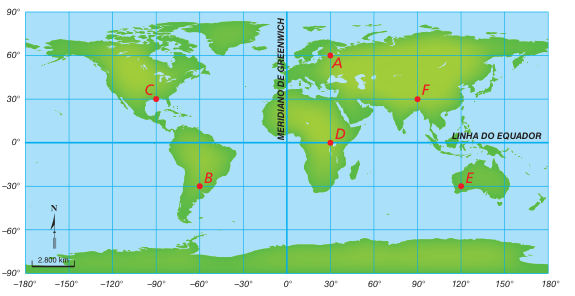
\includegraphics[width=1\linewidth]{figures/2.png}
    \end{figure}

    \begin{enumerate}[I]
      \item Entre os pontos assinalados em vermelho no mapa, determine as coordenadas do ponto:
        \begin{tasks}
          \task assinalado na região que corresponde à América do Sul.
          \task assinalado na região que corresponde à África.
          \task assinalado na região que corresponde à América do Norte.
          \task assinalado na região que corresponde à China.
          \task assinalado na região que corresponde à Europa.
          \task assinalado na região que corresponde à Austrália.
        \end{tasks}
      \item Em que continente está o ponto de latitude $60^\circ$ norte e longitude $120^\circ$ leste?
    \end{enumerate}
\end{enumerate}

\subsection{O conceito de função}

\subsubsection{A noção de função no cotidiano}

Usamos medidas para indicar o comprimento de uma corda, a velocidade de um automóvel, a temperatura 
de uma região, a profundidade de um rio, etc.

Toda carateristíca que pode ser expressa por uma medida é chamada de \textbf{grandeza}.

São exemplos de grandeza: comprimento, área, volume, velocidade, pressão, temperatura, profundidade, 
tempo, massa e razão.

A variação da medida de uma grandeza associada a um objeto depende da variação das medidas  de outras 
grandezas. Por exemplo: o crescimento de uma planta depende do tempo; a taxa de evaporação das águas de um 
rio depende da temperatura; a pressão no mar depende da profundidade. Para estudar essas relações de dependência, 
podemos recorrer a equações matemáticas que relacionem as grandezas envolvidas. 

Para exemplificar, vamos supor que um automóvel percorra um trecho \textit{AB} de uma estrada à velocidade constante de 
80 km/h. 

\begin{figure}[htb!]
  \centering
  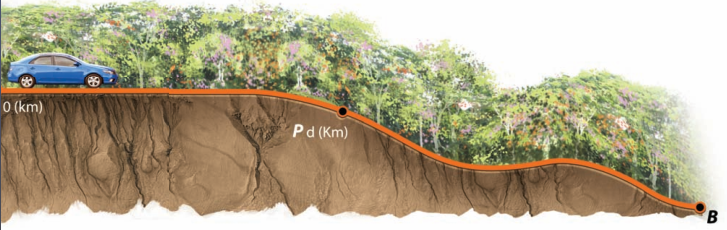
\includegraphics[width=.8\linewidth]{figures/3.png}
\end{figure}

Considerando \textit{A} como ponto de partida, vamos associar a ele a marca 0 km. A cada ponto \textit{P} do trecho \textit{AB},
vamos associar a marca \textit{d} de km, que indica a distância de \textit{A} até \textit{P}, medida ao longo da trajetória. 

Que distância terá percorrido o automóvel após 2 horas da partida?

Como a velocidade do automóvel é constante, 80 km/h, a distância \textit{d} percorrida por ele, em quilomêtro, após 2 horas, será:
\begin{equation*}
  d = 80 \cdot 2 \implies d = 160 \text{ km}
\end{equation*}

Raciocionando de maneira análoga, podemos construir a tabela abaixo, que expressa a distância \textit{d}, percorrida pelo automóvel, após \textit{t}
horas de sua partida. 

\begin{figure}[htb!]
  \centering
  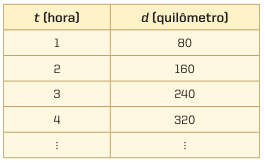
\includegraphics[width=.3\linewidth]{figures/4.png}
\end{figure}

Note que, a cada valor de \textit{t}, associamos um único valor de \textit{d}. Por isso, dizemos que a distância \textit{d} é dada em \textbf{função} do tempo. 

Dessa forma, podemos representar o problema através de uma expressão matemática, que no caso acima corresponde a: 
\begin{equation*}
  d = 80t
\end{equation*}

Observe que a equação substitui a tabela e oferece o cálculo da distância percorrida em qualquer tempo após a partida, e vice-versa. 

Da mesma maneira que relacionamos as grandezas \textit{d} e \textit{t}, podemos relacionar outras grandezas, de modo que a \textbf{cada valor} de uma seja associado \textbf{um único valor}
da outra. Relações como essas são chamadas de funções. 

\dfn{Função}{
  Dizemos que uma variável \textit{y} é dada em \textbf{função} de uma variável \textit{x} se, e somente se, a cada valor de \textit{x} corresponde um único valor de \textit{y}.

  A condição que estabelece a correspondência entre os valores de \textit{x} e \textit{y} é chamada de \textbf{lei de associação}, ou simplesmente lei entre \textit{x} e \textit{y}. Quando 
  possível, essa lei é expressa por uma equação. 
}

\begin{examples}\leavevmode
  \begin{enumerate}
    \item {
        Ao completar o tanque de seu carro em um posto de abastecimento, o motorista olhou para a bomba e observou que havia colocado 26 litros de gasolina e que o total a pagar era 
        R\$ 72.80. 
        \begin{tasks}
          \task Determinar o valor que o motorista teria pago se colocasse apenas 20 litros de gasolina. 
          \task Considerando o montante de gasolina despejada no tanque em cada instante do abastecimento, o preço a pagar é função desse montante? Por quê?
          \task Indicando por \textit{y} o preço a pagar e por \textit{x} os litros de gasolina, formular uma equação que relacione \textit{x} e \textit{y}.
        \end{tasks}

        \textbf{Resolução}
        
        \begin{tasks}
          \task {
            O preço, em real, do litro de gasolina é o quociente de 72.80 por 26, que é 2.80. Logo, por 20 litros de gasolina, o motorista pagaria, em real, $20 \cdot 2.80$, ou seja, 
            R\$ 56.00. 
          }
          \task {
            O preço a pagar é função do montante de gasolina, pois, para cada montante de gasolina despejado no tanque, associa-se um único preço. 
          }

          \task {
            Como o preço do litro de gasolina é R\$ 2.80, o preço \textit{y} de \textit{x} litros é dado por: $y = 2.80 \cdot x$
          }
        \end{tasks}

      }
  \end{enumerate}
  
\end{examples}

\subsubsection{Exercícios Propostos}

\begin{enumerate}[label*=\protect\fbox{\arabic{enumi}}]
  \item A figura \textit{ABCD} é um retângulo tal que: $BD = 6$ cm, $AD = 3$ cm, E é um ponto do lado $\overline{AB}$ e $AE = x$.

    \begin{center}
      
\begin{tikzpicture}
        \tkzDefPoints{0/-3/A, 1.5/-3/E, 6/-3/B, 0/0/D, 6/0/C}
        \tkzDrawPolygon[color=violet, fill=violet!20, thick](A,B,C,D)
        \tkzDrawPoints(A, B, C, D, E)
        \tkzLabelPoint(A){$A$}
        \tkzLabelPoint(B){$B$}
        \tkzLabelPoint[above](C){$C$}
        \tkzLabelPoint[above](D){$D$}
        \tkzLabelPoint(E){$E$}
        \tkzDrawSegment[color=violet, thick](D, E)
        \tkzDrawSegment[color=violet, thick](D, B)
        
      \end{tikzpicture}

    \end{center}
    
    Determine a lei que expressa a área \textit{y} do triângulo \textit{BDE} em função de \textit{x}.

  \item Um metalúrgico recebe R\$ 12.00 por hora trabalhada até o limite de 44 horas semanais, sendo acrescidos 30\% no salário/hora a cada 
    hora que exceder o limite. 

    \begin{tasks}
      \task {Complete a tabela: 
        \begin{figure}[H]
          \centering
          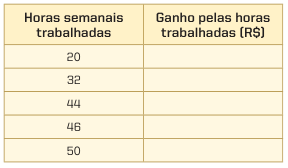
\includegraphics[width=.4\linewidth]{figures/5.png}
        \end{figure} 
      }
      \task O ganho pelas horas trabalhadas é uma função do número de horas semanais trabalhadas? Por quê?
      \task Indicando por \textit{y} o ganho por \textit{x} horas de trabalho semanal, com $x \leq 44$, elabore uma equação que expresse \textit{y} em 
      função de \textit{x}.
      \task Indicando por \textit{y} o ganho por \textit{x} horas de trabalho semanal, com $x > 44$, elabore uma equação que expresse \textit{y} em função de \textit{x}.
    \end{tasks}

  \item Um consumidor comprou um automóvel por R\$ 20000.00, constatando que, ao final de cada ano de uso, o valor de mercado do veículo diminui para 90\% do valor de um ano atrás. 
    Veja na tabela a seguir os valores do automóvel até o final do $2^\circ$ ano. 
    \begin{figure}[H]
      \centering
      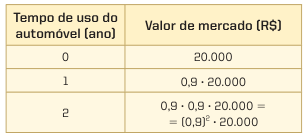
\includegraphics[width=.4\linewidth]{figures/6.png}
    \end{figure}

    \begin{tasks}
      \task Determine o valor do automóvel ao final de 3 anos de uso. 
      \task Determine o valor do automóvel ao final de \textit{x} anos de uso. 
      \task Indicando por \textit{y} o valor de mercado do automóvel com \textit{x} anos de uso, obtenha uma equação que relacione \textit{y} e \textit{x}. 
      \task O valor de mercado do automóvel é dado em função do tempo de uso? Por quê?
    \end{tasks}

  \item Para encher uma piscina, que estava vazia, foi aberta uma torneira cuja vazão é de 26 litros por minuto. 
    \begin{tasks}
      \task Indicando por \textit{y} o volume em litro de água despejada pela torneira em \textit{x} minutos, obtenha uma equação que relacione \textit{x} e \textit{y}.
      \task O volume de água despejada é função do tempo? Por quê?
    \end{tasks}

  \item Em um termômetro, a variação do comprimento da coluna de mercúrio é proporcional à variação da temperatura, obedecendo à razão $\dfrac{8}{5}$; por exemplo,
    o comprimentoda coluna de mercúrio aumenta 8mm para cada $5^\circ C$ de aumento na temperatura; e diminui 8 mm para cada $5^\circ C$ de diminuição na temperatura. 
    Sabe-se que, à temperatura de $0^\circ C$, o comprimento da coluna é 40 mm. 
    \begin{tasks}
      \task Construa uma tabela apresentando os valores, em grau Celsius ($^\circ C$), e os respectivos comprimentos da coluna, em milímetro, com os registros da temperatura 
      variando de $5^\circ C$ em $5^\circ C$ desde $-15^\circ C$ até $15^\circ C$.
      \task O comprimento da coluna de mercúrio é dado em função da temperatura? Por quê?
      \task Formule uma equação que relacione o comprimento do mercúrio com a temperatura.
    \end{tasks}
\end{enumerate}

\subsubsection{Formalização do conceito de função}

\subsubsection*{Relação}

\dfn{Relação entre conjuntos}{
  Dados dois conjuntos não vazios, \textit{A} e \textit{B}, chama-se \textbf{relação} de \textit{A} em \textit{B} qualquer conjunto de pares ordenados ($x,y$) com $x \in A$ e $y \in B$.
}

\begin{example}
  Sendo $A = \{1,2,3,5\}$ e $B = \{-2,-1,0,8,9\}$ a relação \textit{R} de \textit{A} em \textit{B}, que associa um elemento \textit{x} de \textit{A} ao elemento $x - 3$ de \textit{B}, pode 
  ser obtida pela tabela:

  \begin{table}[H]
    \centering
    \begin{tabular}{|s|s|}
      \hline
      \rowcolor{blue!25} $\mathbf{x}$ & $\mathbf{x - 3}$ \\ \hline
      $1$ & $-2$ \\ \hline
      $2$ & $-1$ \\ \hline
      $3$ & $0$ \\ \hline
      $5$ & $?$ \\ \hline
    \end{tabular}
  \end{table}

  Observe que o elemento 5 de \textit{A} não tem correspondente em \textit{B}, pois $5 - 3 = 2$ e 2 não pertence a \textit{B}. Assim a relação \textit{R} é dada por: 
  \begin{equation*}
    R = \{(1,-2),(2,-1),(3,0)\}
  \end{equation*}

  Outra forma de representar essa relação é pelo diagrama de flechas a seguir:

  \begin{center}
    \begin{tikzpicture}
      \tkzText(2,2.2){$R$}
      \draw[violet, thick] (0,0) circle[x radius=1, y radius=2] node[black,circle,fill=violet!30] at (0,1.95) {$A$};
      \draw[violet, thick] (4,0) circle[x radius=1, y radius=2] node[black,circle,fill=violet!30] at (4,1.95) {$B$};
      \tkzDefPoints{0/1.2/1, 0/0.5/2, 0/-0.2/3, 0/-0.9/5}
      \tkzDrawPoints[color=violet](1, 2, 3, 5)
      \tkzLabelPoints[left](1, 2, 3, 5)

      \tkzDefPoints{4/1.2/-2, 4/0.5/-1, 4/-0.2/0, 4/-0.9/8, 4/-1.6/9}
      \tkzDrawPoints[color=violet](-2,-1,0,8,9)
      \tkzLabelPoints[right](-2,-1,0,8,9)

      \draw[->, >=stealth, bend left, shorten <=3pt, shorten >= 3pt] (1.north west) to (-2.north east);
      \draw[->, >=stealth, bend left, shorten <=3pt, shorten >= 3pt] (2.north west) to (-1.north east);
      \draw[->, >=stealth, bend left, shorten <=3pt, shorten >= 3pt] (3.north west) to (0.north east);
    \end{tikzpicture}
  \end{center}

  Para qualquer relação de \textit{A} em \textit{B}:

  \begin{itemize}
    \item o conjunto \textit{A} é chamado de \textbf{conjunto de partida} da relação;
    \item o conjunto \textit{B} é chamado de \textbf{contradomínio} da relação e é simbolizado por \textit{CD(R)};
    \item o conjunto formado pelos elementos de \textit{A} que têm correspondentes em \textit{B}, através de \textit{R}, é 
      chamado de \textbf{domínio} da relação e é simbolizado por \textit{D(R)};
    \item o conjunto formado pelos elementos de \textit{B} que têm correspondentes em \textit{A}, através de \textit{R}, é 
      chamado de \textbf{conjunto imagem} da relação e é simbolizado por $I_m(R)$.
  \end{itemize}

  Para o exemplo anterior, temos $D(R) = \{1,2,3\}$ e $I_m(R) = \{-2,-1,0\}$.

  \begin{center}
    \begin{tikzpicture}
      \tkzText(2,2.2){$R$}
      \draw[violet, thick] (0,0) circle[x radius=1, y radius=2] node[black,circle,fill=violet!30] at (0,1.95) {$A$};
      \draw[violet, thick] (4,0) circle[x radius=1, y radius=2] node[black,circle,fill=violet!30] at (4,1.95) {$B$};
      \draw[teal!100, thick] (-.1,.5) circle[x radius=.4, y radius=1];
      \draw[teal!100, thick] (4.27,.5) circle[x radius=.6, y radius=1];

      \tkzDefPoint(-2.3,1){A}
      \tkzLabelPoint[text width=3.5em, align=center](A){domínio de \textit{R}}
      \draw[->, >=latex, shorten <=3pt, shorten >= 3pt, color=cyan, thick] (-1.7,0.6) to [out=5, in=120](-0.4,1.1);

      \tkzDefPoint(6.3,1){B}
      \tkzLabelPoint[text width=3.5em, align=center](B){imagem de \textit{R}}
      \draw[->, >=latex, shorten <=3pt, shorten >= 3pt, color=cyan, thick] (5.6,0.5) to [in=-50, out=100](4.6,-0.3);

      \tkzDefPoints{0/1.2/1, 0/0.5/2, 0/-0.2/3, 0/-0.9/5}
      \tkzDrawPoints[color=teal](1, 2, 3)
      \tkzDrawPoints[color=violet](5)
      \tkzLabelPoints[left](1, 2, 3, 5)

      \tkzDefPoints{4/1.2/-2, 4/0.5/-1, 4/-0.2/0, 4/-0.9/8, 4/-1.6/9}
      \tkzDrawPoints[color=teal](-2,-1,0)
      \tkzDrawPoints[color=violet](8,9)
      \tkzLabelPoints[right](-2,-1,0,8,9)

      \draw[->, >=stealth, bend left, shorten <=3pt, shorten >= 3pt] (1.north west) to (-2.north east);
      \draw[->, >=stealth, bend left, shorten <=3pt, shorten >= 3pt] (2.north west) to (-1.north east);
      \draw[->, >=stealth, bend left, shorten <=3pt, shorten >= 3pt] (3.north west) to (0.north east);

      \tkzText[text width=8em, align=center](0,-2.5){conjunto de partida}
      \tkzText[text width=8em, align=center](4,-2.3){contradomínio}
    \end{tikzpicture}
  \end{center}

  Também podemos representar essa relação por um gráfico cartesiano, que é formado pelos pontos determinados pelos 
  pares ordenados da relação. Veja abaixo:

  \begin{center}
    \begin{tikzpicture}[scale=.9]
      \tkzInit[xmin=-1, xmax=3, ymin=-2, ymax=1]
      \tkzLabelX[orig=false, font=\footnotesize]
      \tkzLabelY[orig=false, font=\footnotesize]
      \tkzDrawX[left space=1, right space=1]
      \tkzDrawY[up space=1, down space=1]

      \tkzDefPoints{1/-2/A,2/-1/B,3/0/C}
      \tkzDrawPoints[color=violet, scale=1.3](A,B,C)

      \tkzPointShowCoord(A)
      \tkzPointShowCoord(B)
      \tkzPointShowCoord(C)
    \end{tikzpicture}
  \end{center}

  Com base na definição de relação, formalizamos, a seguir, o conceito de função.
\end{example}

\subsubsection*{Função}

Vamos considerar uma relação \textit{f} de \textit{A} em \textit{B} tal que \textbf{qualquer} elemento de \textit{A} esteja associado, através de \textit{f}, a um único elemento de \textit{B}:

\begin{center}
  \begin{tikzpicture}
    \tkzText(2,2.2){$f$}
    \draw[violet, thick] (0,0) circle[x radius=1, y radius=2] node[black,circle,fill=violet!30] at (0,1.95) {$A$};
    \draw[violet, thick] (4,0) circle[x radius=1, y radius=2] node[black,circle,fill=violet!30] at (4,1.95) {$B$};
    \tkzDefPoints{0/1.2/1, 0/0.5/2, 0/-0.2/3, 0/-0.9/5}
    \tkzDrawPoints[color=violet](1, 2, 3, 5)
    \tkzLabelPoints[left](1, 2, 3, 5)

    \tkzDefPoints{4/1.2/-2, 4/0.5/-1, 4/-0.2/0, 4/-0.9/8, 4/-1.6/9}
    \tkzDrawPoints[color=violet](-2,-1,0,8,9)
    \tkzLabelPoints[right](-2,-1,0,8,9)

    \draw[->, >=stealth, bend left, shorten <=3pt, shorten >= 3pt] (1.north west) to (-2.north east);
    \draw[->, >=stealth, bend left, shorten <=3pt, shorten >= 3pt] (2.north west) to (-2.north east);
    \draw[->, >=stealth, bend left, shorten <=3pt, shorten >= 3pt] (3.north west) to (-1.north east);
    \draw[->, >=stealth, bend left, shorten <=3pt, shorten >= 3pt] (5.north west) to (0.north east);
  \end{tikzpicture}
\end{center}

Essa propriedade caracteriza um tipo particular de relação, ao qual damos o nome de \textbf{função} de \textit{A} em \textit{B}. Assim, definimos:

\dfn{Função}{
  Sejam \textit{A} e \textit{B} conjuntos não vazios. Uma relação $f$ de \textit{A} em \textit{B} é \textbf{função} se, e somente se, qualquer elemento de 
  \textit{A} está associado, através de $f$, a um único elemento de \textit{B}. 

  Adotaremos a notação $\mathbf{f: A \rightarrow B}$ para indicar que $f$ é uma função de \textit{A} em \textit{B}.
}

Destacamos que, como uma função $f: A \rightarrow B$ é um tipo particular de relação, temos:

\begin{itemize}
  \item o \textbf{domínio} da função é o próprio conjunto de partida, isto é, $D(f) = A$;
  \item o \textbf{contradomínio} da função é o conjunto $CD(f) = B$;
  \item o \textbf{conjunto imagem} da função é o conjunto $I_m(f) = \{y \in B \text{ | }(x,y) \in f\}$.
\end{itemize}

\begin{examples}\leavevmode
  \begin{tasks}
    \task A relação $g$, abaixo, é uma função de \textit{M} em \textit{N}, pois qualquer elemento de \textit{M} tem, através de $g$, 
      um único correspondente em \textit{N}.
     \begin{center}
        \begin{tikzpicture}
          \tkzText(2,2.2){$g$}
          \tkzText(2,-2.7){$g: M \rightarrow N$}
          \draw[violet, thick] (0,0) circle[x radius=1, y radius=2] node[black,circle,fill=violet!30] at (0,1.95) {$M$};
          \draw[violet, thick] (4,0) circle[x radius=1, y radius=2] node[black,circle,fill=violet!30] at (4,1.95) {$N$};
          
          \tkzDefPoint(0,1.2){A1}
          \tkzDefPoint(0,0.5){A2}
          \tkzDefPoint(0,-0.2){A3}
          \tkzDefPoint(0,-0.9){A4}
          \tkzDrawPoints[color=violet](A1, A2, A3, A4)
          \tkzLabelPoint[left](A1){1}
          \tkzLabelPoint[left](A2){2}
          \tkzLabelPoint[left](A3){3}
          \tkzLabelPoint[left](A4){4}

          \tkzDefPoint(4,1.4){B1}
          \tkzDefPoint(4,0.9){B2}
          \tkzDefPoint(4,0.4){B3}
          \tkzDefPoint(4,-0.1){B4}
          \tkzDefPoint(4,-0.6){B5}
          \tkzDefPoint(4,-1.1){B6}
          \tkzDrawPoints[color=violet](B1, B2, B3, B4, B5, B6)
          \tkzLabelPoint[right](B1){3}
          \tkzLabelPoint[right](B2){4}
          \tkzLabelPoint[right](B3){5}
          \tkzLabelPoint[right](B4){7}
          \tkzLabelPoint[right](B5){8}
          \tkzLabelPoint[right](B6){9}

          \draw[->, >=stealth, bend left, shorten <=3pt, shorten >= 3pt] (A1.north west) to (B1.north east);
          \draw[->, >=stealth, bend left, shorten <=3pt, shorten >= 3pt] (A2.north west) to (B2.north east);
          \draw[->, >=stealth, bend left, shorten <=3pt, shorten >= 3pt] (A3.north west) to (B3.north east);
          \draw[->, >=stealth, bend left, shorten <=3pt, shorten >= 3pt] (A4.north west) to (B4.north east);
        \end{tikzpicture}
      \end{center}

      O domínio $D(g)$, o contradomínio $CD(g)$ e o conjunto imagem $I_m(g)$ dessa função são dados por: 
      \vspace{.3cm}
      \begin{align*}
        D(g) &= M = \{1,2,3,4\} \\
        CD(g) &= N = \{3,4,5,7,8,9\} \\
        I_m(g) &= \{3,4,5,7\}
      \end{align*}

    \task A relação $h$, abaixo, é uma função de \textit{M} em \textit{N}, pois qualquer elemento de \textit{M} tem, 
      através de $h$, um único corresponde em \textit{N}.

      \begin{center}
        \begin{tikzpicture}
          \tkzText(2,2.2){$h$}
          \tkzText(2,-2.7){$h: M \rightarrow N$}
          \draw[violet, thick] (0,0) circle[x radius=1, y radius=2] node[black,circle,fill=violet!30] at (0,1.95) {$M$};
          \draw[violet, thick] (4,0) circle[x radius=1, y radius=2] node[black,circle,fill=violet!30] at (4,1.95) {$N$};
          
          \tkzDefPoint(0,1.2){A1}
          \tkzDefPoint(0,0.5){A2}
          \tkzDefPoint(0,-0.2){A3}
          \tkzDefPoint(0,-0.9){A4}
          \tkzDrawPoints[color=violet](A1, A2, A3, A4)
          \tkzLabelPoint[left](A1){1}
          \tkzLabelPoint[left](A2){2}
          \tkzLabelPoint[left](A3){3}
          \tkzLabelPoint[left](A4){4}

          \tkzDefPoint(4,1.4){B1}
          \tkzDefPoint(4,0.9){B2}
          \tkzDefPoint(4,0.4){B3}
          \tkzDefPoint(4,-0.1){B4}
          \tkzDefPoint(4,-0.6){B5}
          \tkzDefPoint(4,-1.1){B6}
          \tkzDefPoint(4,-1.6){B7}
          \tkzDrawPoints[color=violet](B1, B2, B3, B4, B5, B6, B7)
          \tkzLabelPoint[right](B1){3}
          \tkzLabelPoint[right](B2){4}
          \tkzLabelPoint[right](B3){5}
          \tkzLabelPoint[right](B4){6}
          \tkzLabelPoint[right](B5){7}
          \tkzLabelPoint[right](B6){8}
          \tkzLabelPoint[right](B7){9}

          \draw[->, >=stealth, bend left, shorten <=3pt, shorten >= 3pt] (A1.north west) to (B1.north east);
          \draw[->, >=stealth, bend left, shorten <=3pt, shorten >= 3pt] (A2.north west) to (B1.north east);
          \draw[->, >=stealth, bend left, shorten <=3pt, shorten >= 3pt] (A3.north west) to (B1.north east);
          \draw[->, >=stealth, bend left, shorten <=3pt, shorten >= 3pt] (A4.north west) to (B1.north east);
        \end{tikzpicture}
      \end{center}

      \begin{align*}
        D(g) &= M = \{1,2,3,4\} \\
        CD(g) &= N = \{3,4,5,6,7,8,9\} \\
        I_m(g) &= \{3\}
      \end{align*}

    \task A relação \textit{s}, abaixo, não é função de \textit{M} em \textit{N}, pois existe elemento em \textit{M} (o elemento 4) que não está 
    associado, através de \textit{s}, a algum elemento de \textit{N}.

      \begin{center}
        \begin{tikzpicture}
          \tkzText(2,2.2){$s$}
          \draw[violet, thick] (0,0) circle[x radius=1, y radius=2] node[black,circle,fill=violet!30] at (0,1.95) {$M$};
          \draw[violet, thick] (4,0) circle[x radius=1, y radius=2] node[black,circle,fill=violet!30] at (4,1.95) {$N$};
          
          \tkzDefPoint(0,1.2){A1}
          \tkzDefPoint(0,0.5){A2}
          \tkzDefPoint(0,-0.2){A3}
          \tkzDefPoint(0,-0.9){A4}
          \tkzDrawPoints[color=violet](A1, A2, A3, A4)
          \tkzLabelPoint[left](A1){1}
          \tkzLabelPoint[left](A2){2}
          \tkzLabelPoint[left](A3){3}
          \tkzLabelPoint[left, color=red](A4){4}

          \tkzDefPoint(4,1.4){B1}
          \tkzDefPoint(4,0.9){B2}
          \tkzDefPoint(4,0.4){B3}
          \tkzDefPoint(4,-0.1){B4}
          \tkzDefPoint(4,-0.6){B5}
          \tkzDefPoint(4,-1.1){B6}
          \tkzDefPoint(4,-1.6){B7}
          \tkzDrawPoints[color=violet](B1, B2, B3, B4, B5, B6, B7)
          \tkzLabelPoint[right](B1){3}
          \tkzLabelPoint[right](B2){4}
          \tkzLabelPoint[right](B3){5}
          \tkzLabelPoint[right](B4){6}
          \tkzLabelPoint[right](B5){7}
          \tkzLabelPoint[right](B6){8}
          \tkzLabelPoint[right](B7){9}

          \draw[->, >=stealth, bend left, shorten <=3pt, shorten >= 3pt] (A1.north west) to (B1.north east);
          \draw[->, >=stealth, bend left, shorten <=3pt, shorten >= 3pt] (A2.north west) to (B2.north east);
          \draw[->, >=stealth, bend left, shorten <=3pt, shorten >= 3pt] (A3.north west) to (B3.north east);
        \end{tikzpicture}
      \end{center}

    \task A relação $t$, abaixo, não é função de \textit{M} em \textit{N}, pois existe elemento em \textit{M} ( o elemento 1)
    que está associado, através de $t$, a mais de um elemento de \textit{N}.

      \begin{center}
        \begin{tikzpicture}
          \tkzText(2,2.2){$t$}
          \draw[violet, thick] (0,0) circle[x radius=1, y radius=2] node[black,circle,fill=violet!30] at (0,1.95) {$M$};
          \draw[violet, thick] (4,0) circle[x radius=1, y radius=2] node[black,circle,fill=violet!30] at (4,1.95) {$N$};
          
          \tkzDefPoint(0,1.2){A1}
          \tkzDefPoint(0,0.5){A2}
          \tkzDefPoint(0,-0.2){A3}
          \tkzDefPoint(0,-0.9){A4}
          \tkzDrawPoints[color=violet](A1, A2, A3, A4)
          \tkzLabelPoint[left](A1){1}
          \tkzLabelPoint[left](A2){2}
          \tkzLabelPoint[left](A3){3}
          \tkzLabelPoint[left](A4){4}

          \tkzDefPoint(4,1.4){B1}
          \tkzDefPoint(4,0.9){B2}
          \tkzDefPoint(4,0.4){B3}
          \tkzDefPoint(4,-0.1){B4}
          \tkzDefPoint(4,-0.6){B5}
          \tkzDefPoint(4,-1.1){B6}
          \tkzDrawPoints[color=violet](B1, B2, B3, B4, B5, B6)
          \tkzLabelPoint[right](B1){3}
          \tkzLabelPoint[right](B2){4}
          \tkzLabelPoint[right](B3){5}
          \tkzLabelPoint[right](B4){7}
          \tkzLabelPoint[right](B5){8}
          \tkzLabelPoint[right](B6){9}

          \draw[->, color=red, >=stealth, bend left, shorten <=3pt, shorten >= 3pt] (A1.north west) to (B1.north east);
          \draw[->, color=red, >=stealth, bend left, shorten <=3pt, shorten >= 3pt] (A1.north west) to (B2.north east);
          \draw[->, >=stealth, bend left, shorten <=3pt, shorten >= 3pt] (A2.north west) to (B3.north east);
          \draw[->, >=stealth, bend left, shorten <=3pt, shorten >= 3pt] (A3.north west) to (B4.north east);
          \draw[->, >=stealth, bend left, shorten <=3pt, shorten >= 3pt] (A4.north west) to (B5.north east);
        \end{tikzpicture}
      \end{center}
  \end{tasks}
\end{examples}
